\documentclass[a4paper,12pt]{article}
\usepackage[croatian]{babel}
\usepackage[utf8]{inputenc}
\usepackage[T1]{fontenc}
\usepackage{gensymb}
\usepackage{tikz}
\usepackage{lscape}
\usepackage{amsmath,amsfonts,amssymb,mathrsfs}
\usepackage{fancyhdr,makeidx}
\usepackage{dcolumn,multirow,eucal,hhline,subcaption}
\usepackage{pgfplots,pgfplotstable,colortbl,array}
\usepackage[unicode, hidelinks]{hyperref}
\usepackage{ragged2e}
\usepackage{
epstopdf,
graphicx,tikz,
%pgflibraryshapes,
color,caption,
listings,
dcolumn,
multirow,
array,
booktabs,
picture,
upgreek,
wrapfig,      
cancel,
placeins,
url,
verbatim,
media9,
float,
incgraph
}
\usepackage[nottoc,numbib]{tocbibind}
\usepackage[croatian]{nomencl}
\makenomenclature
\usepgfplotslibrary{units}
\usetikzlibrary{pgfplots.units}
\usetikzlibrary{angles,calc,decorations.pathmorphing,patterns}
\usetikzlibrary{decorations.pathmorphing,decorations.pathreplacing}
\pgfplotstableset{precision=10,set thousands separator={}}
\usepackage{nicefrac}
\hoffset -30 pt
\voffset -50 pt
\textheight = 650 pt
\textwidth = 450 pt
\sloppy
\definecolor{lightgray}{gray}{0.5}
\setlength{\parindent}{0pt}
\usepgfplotslibrary{external}
\usetikzlibrary{pgfplots.external}
\usepgfplotslibrary{external}
\usepackage{lmodern,textcomp}
\usepackage{multimedia}
\headheight = 14 pt
\headwidth = 17 cm
\pagestyle{fancy}


\newcommand{\tikzAngleOfLine}{\tikz@AngleOfLine} %crtanje kuteva
  \def\tikz@AngleOfLine(#1)(#2)#3{%
  \pgfmathanglebetweenpoints{%
    \pgfpointanchor{#1}{center}}{%
    \pgfpointanchor{#2}{center}}
  \pgfmathsetmacro{#3}{\pgfmathresult}%
  }


\fancyfoot[R]{\thepage}
\fancyhead[L]{Marijan Jasak dipl. ing}
\fancyhead[R]{Analiza vrijednosti i njena primjena}
\fancyfoot[L]{}
\fancypagestyle{fancypage}{
    \fancyhf{}
    \footrulewidth=20pt
    %\renewcommand{\headrulewidth}{0pt}
    \renewcommand{\footrulewidth}{0.4pt}
}
\cfoot[]{}
\renewcommand{\thefigure}{\arabic{section}.\arabic{subsection}.\arabic{figure}}
\makeindex
\numberwithin{figure}{section}

\setlength\parindent{24pt}
\begin{document}

\begin{titlepage}
\begin{titlepage}
  \null\vfill

  \begin{center}

  {\huge\bfseries Analiza vrijednosti \\ i njena primjena}
  \vskip 2cm
  
  \end{center}

\vfill


\begin{tabular}[t]{c}
Marijan Jasak dipl. ing.\\ sour "Rade Končar" \\ Zagreb
\end{tabular}
\hfill
\end{titlepage}
\end{titlepage}
\section*{Analiza vrijednosti i njena primjena}
Živimo u doba naglog razvoja znanosti. Znanosti, koja dovodi do novih materijala i tehnologija, a time i do novih načina proizvodnje. Na taj način se otvaraju fantastične mogučnosti usavršavanja postojećih proizvoda. Dodamo li tome bujnu ljudsku maštu, otvaraju se daljnje perspektive i stvaranja novih proizvoda. Funkcije tih proizvoda ovise o našim, ljudskim, potrebama i intuiciji predlagaća za potrebe sutradašnjice.\par
Danas već možemo proizvesti skoro sve što je netko zamislio. Ali cilj proizvodnje nije u tome da se nešto proizvodipod svaku cijenu, nego:
\begin{center}
POTREBNO JE PROIZVESTI PROIZVOD UZ MINIMALNE TROŠKOVE!
\end{center}
\noindent Tako proizvod treba:
\begin{itemize}
	\item u potpunosti ispuniti funkcije zbog kojih se proizvodi
	\item biti kvalitetno postojan
	\item udovoljiti zahtjevima na tržištu po izgledu savremenosti i količini
	\item biti jeftiniji od konkurentskih proizvoda iste funkcije i kvalitete.
\end{itemize}
\noindent Udovolji li proizvod ove postavke, održat će se na tržištu. Ako su i vlastiti troškovi proizvodnje manji od cijene koju diktira tržište, proizvod stvara i akumulaciju~(Slika \ref{Slika1}). \par
Djelovati na troškove proizvodnje je moguće i na samom početku stvaranja, kako ideje o proizvodu, tako i o načinu proizvodnje. \par
Kod prozivodnje se misli na sve faze razvoja proizvoda počevši od ideje, preko konstrukcije do lansiranja proizvoda na tržište. U tu grupu spada i izrada tehničko ekonomskih alaniza postoječih proizvoda za iznalaženje najboljeg proizvodng nivoa. \par
Kod proizvodnje se misli na sve faze eventualnog projektiranja i izgradnje nove tvornice, koja će proizvoditi predviđeni proizvod, odnosno, otkrivati mogučnosti smanjenja vlastitih troškova proizvodnje u postoječoj proizvodnji. Traženje najpovoljnijeg riješenja proizvodnje nekog proizvoda nije mali i jednostavan zadatak. To je kompleksni problem, koji se praktiči mjenja iz dana u dan. Jer, ONO ŠTO JE JUČER BILO NAJBOLJE, DANAS JE JOŠ DOBRO, A SUTRA VIŠE NEĆE ZADOVOLJAVATI!

\begin{figure}
\centering
\input{formiranje_cijene} 
\caption{Formiranje cijene proizvoda na tržištu}\label{Slika1}
\end{figure}
\FloatBarrier
\par
Ovo nas upučuje na nova i daljnja istraživanja vezana uz svaki proizvod. Uz svaki \textbf{trošak}! A svagdje gdje nastaje trošak potrebno je obaviti istraživanja, dali je on \underline{najmanji}, to jest neophodno potreban u tom iznosu.\par
Kod proizvodnje treba potrošiti od proizvodnog načela:
\begin{center}
"Ne raditi toliko dobro koliko je moguće, nego, toliko dobro koliko je potrebno!"
\end{center}
\par
Da bi predvidljeli buduće troškove ili obavili analizu sadašnjih, koristimo se metodama \textbf{ANALIZE VRIJEDNOSTI}. Postavlja se pitanje: ŠTO JE ANALIZA VRIJDNOSTI?\\
Odgovor je vrlo jednostavan:\par
Analiza vrijednosti je sistematska metoda rada, koja s velikom vjerojatnošću određuje optimalna riješenja a datim uvijetima proizvodnje i stupnju saznanja. \\
Osnovne značajke metode su:
\begin{itemize}
\item Interdisciplinarni timski rad, kao najefikasnije stvaralačko stedstvo naučno tehničkog napretka, jer učinak timskog rada znatno je veći od sume pojedinačnih učinaka istih članova tima.
\begin{center}
"Više ljudi, ne samo što više vide, nego i drugačije vide isti problem"
\end{center}
\item Postupak rada po metodama analize vrijednosti odvija se točno po unaprijed  određenom planu kadkada i u odvojenim fazama.
\item Postupak realizacije analize vrijednosti u osnovi je neovisan o vrsti objekata koji analiziramo (proizvod, proizvodni proces, organizacija svih vrsti poslova itd.), o fazi razvoja, planiranja ili realizacije.
\end{itemize}
\par
Obim radova ovistan je od konkretnog zadatka, ali uvijek prema unaprijed postavljenom cilju!
\par
Prema DIN 69910, plan rada na analizi vrijednosti podijeljen je u 6 (šest) osnovnih faza s po nekoliko faza:
\begin{enumerate}
\item \textbf{ABC ANALIZA} - koristi se kod izbora objekata za analizu vrijednosti
\item \textbf{TEHNIKA MREŽNOG PLANIRANJA} - koristi se kod izrade plana radova
\item \textbf{VREDNOVANJE FUNKCIJE} - koristi se kod izrade kalkulacija pojedinih funkcija
\item \textbf{METODE ISTRAŽIVANJA IDEJA} - unutar čega se koristi
\begin{itemize}
\item Brainstorming - spontano i nekontrolirano iznošenje ideja za iznalaženje zadovoljenja tražene funkcije. Postoji čitav niz uzroka, koji nas sprečavaju, da iznesemo svoje ideje pred grupu ljudi bez opterećenja. Među te uzroke spadaju:
\begin{itemize}
\item navike i stavovi; želja za dostojanstvom
\item bojazan, da ne ispadnemo smješni; tradicija
\item bojazan od raznih komplikacija koje proizlaze iz konflikata s okolinom, ukoliko predložimo nešto suprotno; rutinski duh stručnjaka
\item bojazan od kritičkog duha, koji se kod skupljanja ideja mora suzbit - NESMIJEMO KRITIZIRATI NITI JEDNU IDEJU!; itd.
\end{itemize}  
\item Metoda 653 - lančano dopisivanje ideja šestorice (6) sudionika kroz pet (5) minuta po tri (3) ideje.
\item Ostale metode. 
\end{itemize}
\item \textbf{METODE UPITNE LISTE - PROVOKATIVNA PITANJA} - koristi se kod istraživanja mogučih riješenja. Bit ove metode je, da vođa tima postavlja grupi pitanja u vezi problema koji se promatra. Odgovori na pitanja u vezi problema koji se promatra. Odgovori na pitanja su DA ili NE. Na odgovor DA, postavlja se pitanje KAKO?.  Ako je odgovor NE, postavlja se pitanje ZAŠTO?. Evo i nekoliko uobičajenih pitanja:
\begin{center}
\begin{enumerate}
\item Dali su potrebne sve funkcije koje proizvod obnavlja?
\item Dali funkcija može preuzeti neki drugi dio?
\item Može li se koristiti jeftiniji materijal?
\item Mogu li se koristiti standardni dijelovi?
\item Možemo li povečati tolerancije?
\item Možemo li smanjiti otpad ili škart?
\item Možemo li neke radne operacije eliminirati?
\item Možemo li koristiti postojeće alate?
\item Možemo li promijeniti način površinske obrade?
\item Možemo li pronači povoljnijeg dobavljača?
\item Dali naš konkutrent to nabavlja povoljnije?
\item Možemo li koristiti jeftinije radne operacije? itd.
\end{enumerate}
\end{center} 
\end{enumerate}

\begin{table}[]
\centering
\label{my-label}
\begin{tabular}{|l|l|}
\hline
\begin{tabular}[c]{@{}c@{}} FAZE I PODFAZE AV \end{tabular} & \begin{tabular}[c]{@{}c@{}} KARAKTERISTIČNA PITANJA \end{tabular}                                                                                                                                                                                          \\ \hline
\begin{tabular}[c]{@{}l@{}}1. Pripremi radovi\\ 1.1. Izbor objekata AV i postavljanje zadataka.\\ 1.2. Određivanje kvantificiranog cilja.\\ 1.3. Formiranje tima.\\ 1.4. Izrada plana i troškova.\end{tabular} &                                                                                                       \\ \hline
\begin{tabular}[c]{@{}l@{}}2. Utvrđivanje sadašnjeg stanja \\ 2.1. Opis objekata AV i prikupljanje informacija.\\ 2.2. Opis funkcija.\\ 2.3. Određivanje troškova.\end{tabular}                              & \begin{tabular}[c]{@{}l@{}}Što je to?\\ Koja mu je funkcija?\\ Što radi?\\ Koliko košta?\end{tabular} \\ \hline
\begin{tabular}[c]{@{}l@{}}3. Analiza sadašnjeg stanja\\ 3.1. Analiza funkcija - ciljne funkcije.\\ 3.2. Analiza troškova - ciljni troškovi.\end{tabular}                                                   & \begin{tabular}[c]{@{}l@{}}Kako radi?\\ Što treba raditi?\\ Koliko smije koštati?\end{tabular}        \\ \hline
\begin{tabular}[c]{@{}l@{}}4. Određivanje alternativnih rješenja\\ 4.1. Istraživanje svih mogućih riješenja.\end{tabular}                                                                                  & \begin{tabular}[c]{@{}l@{}}Koje bi drugo riješenje zadovoljavalo\\ traženu funkciju?\end{tabular}     \\ \hline
\begin{tabular}[c]{@{}l@{}}5. Vrednovanje alternativa\\ 5.1. Vrednovanje realnosti primjene.\\ 5.2. Vrednovanje rentabilnosti.\end{tabular}                                                                 & \begin{tabular}[c]{@{}l@{}}Kako vrši funkciju?\\ Koliko košta?\end{tabular}                           \\ \hline
\begin{tabular}[c]{@{}l@{}}6. Izbor optimalnog riješenja, prijedlog i realizacija\\ 6.1. Izbor optimalnog riješenja.\\ 6.2. Izrada prijedloga.\\ 6.3. Ostvarivanje prijedloga.\end{tabular}                  &                                                                                                       \\ \hline
\end{tabular}
\end{table}
\FloatBarrier
Odgovori na postavljena pitanja su odgovori analize vrijednosti i to je ono što čini analizu vrijednosti različitom od drugih metoda, odnosno sistema za iznalaženje optimalnih riješenja.\\ 
U pojedinim fazama, odnosno predfazama rada na analizi vrijednosti, koristimo već dobro poznate tehnike. Tu spadaju:
\begin{enumerate}
\item \textbf{PROUČAVANJE PROIZVODA KONKURENCIJE} - koristi se također kod istraživanja mogućih riješenja. Nije potrebno OTKRIVATI TOPLU VODU! Primjena dobrih riješenja konkurentskih proizvoda, nije krađa ideja, niti je kopiranje, čega bi se trebalo stidjeti. To je razionalno trošenje sredstava i vremena. Pametno korišenje saznanja drugih, najjeftiniji je način prikupljanja ideja.
\item \textbf{TEST VRIJEDNOSTI} - koristi se na kraju analize svakog objekta da se još jednom provjeri predloženo riješenje i ustanovi dali je  u skladu s postavljenim ciljevima i postupkom analize vrijednosti, tj. dali objekt ispunjava sve funkcije u potrebnoj kvaliteti i pouzdanosti uz minimalne troškove. Pitanja u testu vrijednosti definirao je tvorac analize vrijednosti, amerikanac L.D.Miles. 
\end{enumerate}
Izoliran rad pojedinih stručnih grupa i pojedinac, iako svaki za sebe savršen, nemože i neće donjeti optimalno riješenje. Takovim radom dolazimo do proizvoda, postupka, ili organizacije, koja će tehnički biti na veoma visokom nivou, možda predobra, ali sigurno preskupa, jer je opterečena nepotrebnim troškovima.\\
Prema dosadašnjem iskustvu na primjeni analize vrijednosti u svijetu i kod nas, pokazalo se, da su proizvodi prosječno opterečeni s približno 20\% nepotrebnih troškova. Ti se suvišni troškovi penju i do 40\% kod nekih, na brzinu razvijenih i usvojenih proizvoda, koje je tražilo tržište. Prisutstvo takovih nepotrebnih troškova u tako visokom postotku potvrđuju da je primjena analize vrijednosti potrebna i ispravna.\par
Metode analize vrijednosti prvi puta u Jugoslaviji su primijenjene u SOUR"Rade Končar" - Zagreb, negdje 1960. godina. Prve pisane materijale o analizi na našem jeziku napisali su stručnjaci "Rade Končara". Ipak moramo konstatirati da primjena metode nije našla svoje mjesto u djelatnosti cijelog SOUR-a. Neinformiranost užeg rukovodstva i premali broj školovanih stručnjaka osnovni su razlozi slabe primjene analize vrijednosti. Djelatnost primjene analize vrijednosti unutra SOUR "Rade Končar" obavlja se u ODUR - Inženjering za investicijsku izgradnju i to u službi za razvoj proizvodnje. Treba naglasiti da su kapaciteti nesrazmjerno mali u odnosu na važnost i potrebu takove djelatnosti. Dodamo li tome, da je kod samo jednog proizvoda ostvarena ušteda od 15.000.000 dinara, vidljiva je opravdanost postojanja takove djelatnosti. Sada se već pomalo formiraju timovi i u drugim sredinama SOUR, ali je još to uvijek premalo i pomalo stihijsko. \par
Da bi analiza vrijedosti bila efikasna mora biti postavljena na potreban organizacijski nivo, tj. ona mora biti prištabski organ rukovodstva, što bi šematski odgovaralo:
\begin{figure}
\centering
\input{poslovnamapa} 
\caption{Formiranje cijene proizvoda na tržištu}\label{Slika1}
\end{figure}
Analiza vrijednosti, kao specifična djelatnost, dati će tek u takvoj organizaciji dobre rezultate \underline{ako ima i}:
\begin{itemize}
\item \textbf{BEZREZERVNU PODRŠKU I AKTIVNE ORGANE UPRAVLJANJA}(bez toga nema smisla uvoditi analizu vrijednosti u svoj poslovni sistem) i
\item \textbf{DOBRU PRIPREMU} - u što spada izobrazba kadrova, koji će u fazi uvođenja i primjena raditi aktivno na analizi vrijednosti.
\end{itemize}
\newpage
\section*{Prikaz obavljenih radova na analizi vrijednosti}
Dosada obavljene analize vrijednosti bile su provedene isključivo na proizvodima i to pretežno na postoječim proizvodima. Želja je bila da se smanje troškovi proizvodnje najmanje za 15\%. Rezultati su bili premašeni.\par
Na sljedečem primjeru želio bih Vam pokazati način pristupa radu na analizi nekog proizvoda.\par
Zahtjev SOUR PROIZVODNJE DIZALA bio je da se obavi analiza vrijednosti na OSOBNOM DIZALU 4500kN, 10 stanica, 10 ulaza, s brzinom 0,8/0,2 m/sek. Osnovni djelovi tog dizala su:
\FloatBarrier
\begin{table}[h!]
\centering
\begin{tabular}{lll}
\textbf{Naziv sklopa}             & \textbf{Postotni dio}  & \textbf{Redni broj za ABC} \\
1. Poluautomatska vrata  & 13,58         & 2                 \\
2. Vrata strojarnice     & 1,06          & 13                \\
3. Vodilice              & 13,08         & 3                 \\
4. Kabina                & 9,47          & 4                 \\
5. Okvir kabine          & 7,82          & 7                 \\
6. Okvir utega           & 4,65          & 8                 \\
7. Pogonski stroj        & 23,79         & 1                 \\
8. Ograničivać brzine    & 1,26          & 12                \\
9. Užad                  & 2,12          & 10                \\
10. Kutije               & 2,1           & 11                \\
11. Grupa za upravljanje & 9,05          & 6                 \\
12. Instalacije          & 9,17          & 5                 \\
13. Ulje                 & 0,08          & 15                \\
14. Ambalaža             & 0,51          & 14                \\
15. Transport            & 2,24          & 9                 \\ \hline
                         & Ukupno 100,00 &                  
\end{tabular}
\end{table}
Na osnovu te podjele izrađen je diagram ABC analize (Slika!\ref{analiza}).

\begin{figure}
  \centering
    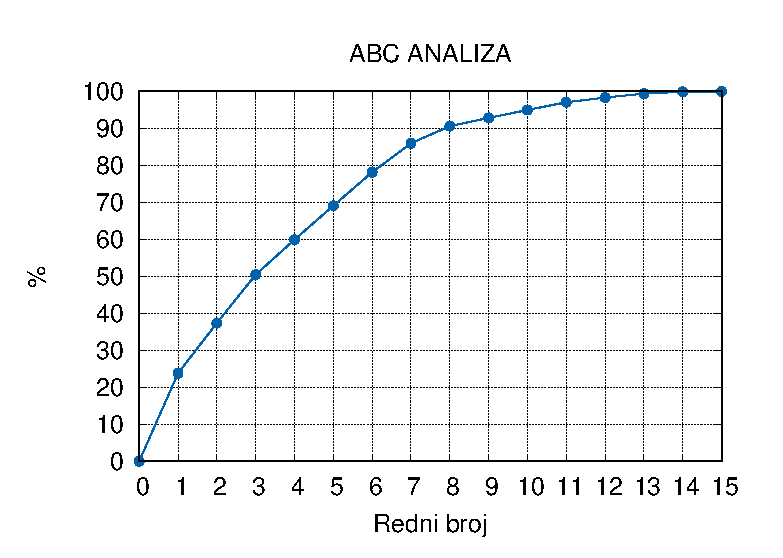
\includegraphics[width=0.8\paperwidth]{abcAnaliza.eps}
    \caption{ABC analiza}
    \label{analiza}
\end{figure}
\FloatBarrier

ABC analiza nas upučujue da prvo moramo obaviti analizu pogonskog stroja. Pogonski stroj smo zatim rastavili na njegove podsklopove, a neke od podsklopova na elemente (prema šemi).\par
Nakon rastavljanja \underline{postolja} uočeno je da 52,7\% vrijednosti otpada na otklonsku užnicu, čija funkcija, \underline{odmicanje užeta} do simetrale otvora za kabinu. Taj podatak je bio začuđujući i za same konstruktore. Nakon rastavljanja otklonske užnice na elemente upada u oči da su kuglični ležajevi preskupi. Zamjenjeni su na postoječim konstrukcijama jeftinijim.\par
Analizom smo išli tako daleko da smo u novim konstrukcijama, uvođenjem standardnoh izmjera kabine, otklonsku užnicu izbacili.\par
Drugi element po utjecajnosti u postolju komplet je nosač stroja. Rastavivši ga na elemente, definirali smo funkciju svakog elementa. Uzevši u obzir postolje elektromotora, koji nosi elektromotor, proizlazi funkcija poprečnih nosača, da oni nose uzdužne nosače, koji opet nose nosač elektromotora. To nas je uputilo da pokušamo neke od nosača zamijeniti ili eliminirati. Konkretno, nosač elektromotora možemo eliminirati uvođenjem prirubnog motora.\par
Ovdje smo stali s analizom postoječeg riješenja. Konstatirano je da treba izrazit sasvim novu koncepciju pogonskog stroja i to:
\begin{itemize}
\item s prirubnim elektromotorom
\item bez otklonske užnice
\item uvođenjem dvostrukog regulatora brzine.
\end{itemize}
Sve je to sada u fazi konstruiranja i očekuje se 25\% jeftiniji pogonski stroj.

\begin{landscape}
\begin{figure}
\input{shema}
\caption{Šema rastavljanja pogonskog stroja.}\label{Slika2}
\end{figure}
\end{landscape}
\clearpage
\begin{figure}[!h]
\centering
\includegraphics[scale=0.22]{../ObradaMetala/Dino/image_62.png}
\end{figure}
\FloatBarrier

Želio bih Vam pokazati jedan veoma interesantan detalj koji se pojavio radeći na analizi vrijednosti. Interesantan i karakterističan u ovakvom radu. Radi se o vijeku \textbf{regulatora zraka} na uljnim pećima.\par

Vijak služi za držanje zaklopke regulatora zraka u željenom položaju, a omogućuje i postavlja zaklopke, ovisno o svojstvima dimnjaka, u drugi položaj. Koriste se dva vijka.\par
Kod izrade ovog detalja konstrukter se pridržavao određenih pravila i to:
\begin{itemize}
\item vijak mora biti standardni.
\item vijak mora imati narovašenu glavu, jer se uvija rukom
\item vijak mora imati površinsku zaštitu da ne hrđa
\item vijak mora držati zaklopku u određenom položaju, tj. mora biti dobro dimenzioniran.
\end{itemize}
Držeći se gornjih postavki, konstrukter je izabrao:

\textbf{Vijak M3x6 JUS M.81.200} svijetlo poniklan. Nabavna cijena je 0,65 din/kom a izrađuje se po narudžbi. Godišnja potreba je 170 000 kom.
\begin{wrapfigure}{l}{0.5\textwidth}
  \vspace{-20pt}
  \begin{center}
    \input{vijak}
  \end{center}
  \vspace{-20pt}
  \vspace{-10pt}
\end{wrapfigure}
U ABC analizi uljne peći, promatrani vijak je bio u grupi C. Odma je bilo konstatirano da je \textbf{preskup za ono što radi!} Tim je odlučio da ovom vijku posveti nekoliko minuta, jer su godišnji troškovi nabavke tog vijka 110.500 dinara. Analizirajući sklop u koji je vijak ugrađen, ustanovljeno je sljedeće:
\begin{enumerate}
\item Funkcija tog vijka je da - drži zaklopku
\item Vrijednost funkcije - procijenjena na 0,10 dinara
\item Sadašnja vrijednost - 1,30 dinara.
\end{enumerate} 
Iz toga proizlazi da se može očekivati ušteda od $\approx$100.000 dinara. Ekonomska opravdanost troškova na analizi vrijednsoti je 10\%, pa se stoga mogu planirati troškovi od 10.000 dinara. Neka su troškovi svakog člana tima $\approx$50 d/h, za analizu možemo utrošiti $\approx$200 h.
\begin{center}
Zaključak tima - ANALIZIRATI VIJAK
\end{center}
Osnovna misao je - zamjeniti vijak jeftinijim\\
Reagiranja - otpor konstrukcije i servisa\\
Primjenjena metoda - korištenje testova (chech listi) - RUŠITI PREPREKE, PRIMJENJITI PROVOKATIVNA PITANJA!

\begin{table}[]
\centering
\begin{tabular}{|l|l|}
\hline
\textbf{Pitanje}                                                                                              & \textbf{Odgovor}                                                                                                                                                                                                                                                                                      \\ \hline
1. Dali mora biti poniklan?                                                                          & DA!                                                                                                                                                                                                                                                                                          \\ \hline
2. Zašto?                                                                                            & Inače korodira                                                                                                                                                                                                                                                                               \\ \hline
3. Dali to smeta funkciji?                                                                           & NE!                                                                                                                                                                                                                                                                                          \\ \hline
4. Kome smeta?                                                                                       & Izgledu.                                                                                                                                                                                                                                                                                     \\ \hline
5. Dali se to vidi u svakodnevnoj upotrebi?                                                          & \begin{tabular}[c]{@{}l@{}}NE! Nalazi se u zadnjem \\ dijelu peći okrenutom\\ prema zidu.\end{tabular}                                                                                                                                                                                       \\ \hline
6. Tko to vidi?                                                                                      & Radnik pri montaži i serviser.                                                                                                                                                                                                                                                               \\ \hline
7. Kako izgledaju ostali dijelovi oko tog vijka?                                                     & \begin{tabular}[c]{@{}l@{}}U upotrebi su to prljavi \\ nezaštičeni limovi uprljani \\ uljem i prašinom.\end{tabular}                                                                                                                                                                         \\ \hline
8. Zašto onda vijak mora biti poniklan?                                                              & \begin{tabular}[c]{@{}l@{}}Konstatacija: VIJAK NEMORA\\ BITI SJAJNO PONIKLAN!\end{tabular}                                                                                                                                                                                                   \\ \hline
\begin{tabular}[c]{@{}l@{}}9. Dali vijak mora imati takav oblik s \\ nareckanom glavom?\end{tabular} & DA!                                                                                                                                                                                                                                                                                          \\ \hline
10. Zašto?                                                                                           & \begin{tabular}[c]{@{}l@{}}Da se može odviti i ponovno \\ zavrtiti rukom prilikom\\ regulacije zaklopke.\end{tabular}                                                                                                                                                                        \\ \hline
11. Tko vrši regulaciju?                                                                             & Naš servis.                                                                                                                                                                                                                                                                                  \\ \hline
12. Kako često?                                                                                      & \begin{tabular}[c]{@{}l@{}}Pitati servis, a odgovor glasi:\\ Samo iznimno u slučajevima kada \\ dimnjak nema dovoljan podtlak.\end{tabular}                                                                                                                                                  \\ \hline
13. Kako se vrši regulacija?                                                                         & \begin{tabular}[c]{@{}l@{}}Otpuštanjem vijka; Zakretanjem\\ okvira. Stezanje vijka.\end{tabular}                                                                                                                                                                                             \\ \hline
14. Dali je kod toga uopće potrebno odviti vijak?                                                    & \begin{tabular}[c]{@{}l@{}}Probama na pećima je konstatirano: \\ VIJAK NETREBA OTPUSTITI!\\ Naime, pritiskom na gornji ili\\ donji dio okvira, zaklopka se \\ može postaviti u željeni položaj, bez\\ otpuštanja vijka. Konstatacija:\\ VIJAK NEMORA IAMTI OVAKAV\\ OBLIK GLAVE\end{tabular} \\ \hline
\end{tabular}
\end{table}
\FloatBarrier
Zaključak: Može se koristiti običan vijak s cilindričnom glavom. Predloženo je sljedeće riješenje:
\begin{itemize}
\item Vijak, M3x6 JUS MB1.103. Moguće ga je kupiti u trgovini uz cijenu 0,03 din/kom.
\end{itemize}
\begin{wrapfigure}{r}{0.4\textwidth}
  \vspace{-20pt}
  \begin{center}
    \input{vijakx}
  \end{center}

\end{wrapfigure}
\FloatBarrier
Iz toga proizlazi ušteda:
\begin{center}
170 000 [kom/god] x (0,65 - 0,03)[din/kom] = 105 400 [din/god]
\end{center}
Svedeno u postotke, sniženje troškova je:
\begin{center}
\begin{equation*}
\frac{\mathsf{ušteda}}{\mathsf{sadašnji\: troškovi}} \cdot 100 = \frac{0,62}{0,65} \cdot 100 = 94,5\:
\%
\end{equation*}
\end{center}
Troškovi analize iznose:
\begin{itemize}
\item Rad tima 5x2 (h) = 10 h
\item Konzultacije sa servisom 8 h
\item Probe u radioni i servisu 5 x 1 h = 5h
\item Ostalo 10 h
\end{itemize}
Uz jedinične troškove od 50 din/h nastali troškovi od 33 [h] x 50 [din/h] = 1650 din što je znatno ispod predviđenih 10 000 dinara. Ova analiza je obavljenja 1971. godine.\par
Od zanačajnih radova još bi spomenuo:
\begin{itemize}
\item Zamjena kučišta serijskih elektromotora od sivog ljeva na kučišta od tlačnog lijeva. 
\item Zamjena duboko izvačene ventilatorske kape elektromotora s kapom izrađenom of termoplasta
\item razvoj i proizvodnja novog plinskog releja (Bueholz)
\item nova familija transformatorskih kotlova za cijelu gamu serijskih transformatora prijelazom od radijatora i cijevnih lira na valovitu kanstrukciju uz istodobno pojednostavljenje cijelog kotla, itd.\\


\vfill\noindent
\begin{tabular}[t]{@{}l} 
  Zagreb 1972.
\end{tabular}
\hfill% move it to the right
\begin{tabular}[t]{l@{}}
Marijan Jasak dipl. inž.\\
SOUR "Rade Končar"\\
41000 Zagreb\\
Fallerovo Šetalište 22.
\end{tabular}

\end{itemize}






\end{document}